\documentclass[11pt]{article}\usepackage[]{graphicx}\usepackage[dvipsnames]{xcolor}
% maxwidth is the original width if it is less than linewidth
% otherwise use linewidth (to make sure the graphics do not exceed the margin)
\makeatletter
\def\maxwidth{ %
  \ifdim\Gin@nat@width>\linewidth
    \linewidth
  \else
    \Gin@nat@width
  \fi
}
\makeatother

\definecolor{fgcolor}{rgb}{0.345, 0.345, 0.345}
\newcommand{\hlnum}[1]{\textcolor[rgb]{0.686,0.059,0.569}{#1}}%
\newcommand{\hlsng}[1]{\textcolor[rgb]{0.192,0.494,0.8}{#1}}%
\newcommand{\hlcom}[1]{\textcolor[rgb]{0.678,0.584,0.686}{\textit{#1}}}%
\newcommand{\hlopt}[1]{\textcolor[rgb]{0,0,0}{#1}}%
\newcommand{\hldef}[1]{\textcolor[rgb]{0.345,0.345,0.345}{#1}}%
\newcommand{\hlkwa}[1]{\textcolor[rgb]{0.161,0.373,0.58}{\textbf{#1}}}%
\newcommand{\hlkwb}[1]{\textcolor[rgb]{0.69,0.353,0.396}{#1}}%
\newcommand{\hlkwc}[1]{\textcolor[rgb]{0.333,0.667,0.333}{#1}}%
\newcommand{\hlkwd}[1]{\textcolor[rgb]{0.737,0.353,0.396}{\textbf{#1}}}%
\let\hlipl\hlkwb

\usepackage{framed}
\makeatletter
\newenvironment{kframe}{%
 \def\at@end@of@kframe{}%
 \ifinner\ifhmode%
  \def\at@end@of@kframe{\end{minipage}}%
  \begin{minipage}{\columnwidth}%
 \fi\fi%
 \def\FrameCommand##1{\hskip\@totalleftmargin \hskip-\fboxsep
 \colorbox{shadecolor}{##1}\hskip-\fboxsep
     % There is no \\@totalrightmargin, so:
     \hskip-\linewidth \hskip-\@totalleftmargin \hskip\columnwidth}%
 \MakeFramed {\advance\hsize-\width
   \@totalleftmargin\z@ \linewidth\hsize
   \@setminipage}}%
 {\par\unskip\endMakeFramed%
 \at@end@of@kframe}
\makeatother

\definecolor{shadecolor}{rgb}{.97, .97, .97}
\definecolor{messagecolor}{rgb}{0, 0, 0}
\definecolor{warningcolor}{rgb}{1, 0, 1}
\definecolor{errorcolor}{rgb}{1, 0, 0}
\newenvironment{knitrout}{}{} % an empty environment to be redefined in TeX

\usepackage{alltt}
\usepackage[utf8]{inputenc}
\usepackage[T1]{fontenc}
\usepackage{lmodern}
\usepackage{amsmath, amssymb, amsthm, graphicx, physics}
\usepackage{enumitem}
\usepackage{geometry}
\usepackage[dvipsnames]{xcolor}
\definecolor{EvanPink}{rgb}{0.85, 0.13, 0.55}
\usepackage[colorlinks=true,
            linkcolor=OliveGreen,
            urlcolor=EvanPink,
            citecolor=OliveGreen]{hyperref}
\usepackage{cleveref}
\usepackage{etoolbox}
\newenvironment{solution}{%
  \par\noindent\textit{Solution.}\ }{\qed}
\newtheoremstyle{problemstyle}
  {1em}   
  {1em}   
  {}      
  {}      
  {\bfseries} 
  {.}     
  {0.5em} 
  {}      
\theoremstyle{problemstyle}
\newtheorem{problem}{Problem}[section]
\crefname{problem}{Problem}{Problems}
\Crefname{problem}{Problem}{Problems}
\def\bN{\mathbb{N}}
\def\bR{\mathbb{R}}
\def\bZ{\mathbb{Z}}
\def\bQ{\mathbb{Q}}
\def\mM{\mathcal{M}}
\def\mR{\mathcal{R}}
\def\mN{\mathcal{N}}
\def\mE{\mathcal{E}}
\def\mA{\mathcal{A}}
%%%%%%%%%%%%%%%Setting Page Sizes %%%%%%%%%%%%
\setlength{\parindent}{0in}
\setlength{\parskip}{\baselineskip}
\setlength{\textheight}{9in}
\setlength{\textwidth}{6.3in}
\setlength{\topmargin}{-0.6in}
\setlength{\evensidemargin}{-.5in}
\setlength{\oddsidemargin}{0in}
%%%%%%%%%%%%%%%%%%%%%%%%%%%%%%%%%%%%%%%%%%%

%%%%%%%%%%%%To make R commands appear in different Color%%%%%%%%%%
\usepackage{color}
\usepackage{fancyvrb} % Verbatim
\usepackage{Sweave} % for R code
\usepackage{color}
\definecolor{codecolor}{RGB}{114,12,112}
\DefineVerbatimEnvironment{Sinput}{Verbatim}{formatcom=\color{codecolor}}
\DefineVerbatimEnvironment{Soutput}{Verbatim}{formatcom=\color{codecolor}}
\DefineVerbatimEnvironment{Scode}{Verbatim}{formatcom=\color{codecolor}}
\DefineVerbatimEnvironment{Sin}{Verbatim}{formatcom=\color{codecolor}}
\DefineVerbatimEnvironment{Sout}{Verbatim}{formatcom=\color{codecolor}}
%%%%%%%%%%%%%%%%%%%%%%%%%%%%%%%%%%%%%%%%%%%%%%%%%%%%%%%%%%%%%%%%

\IfFileExists{upquote.sty}{\usepackage{upquote}}{}
\begin{document}

{\bf Arkaraj Mukherjee: }
{\bf Worksheet 4-2}
\\
\begin{knitrout}
\definecolor{shadecolor}{rgb}{0.969, 0.969, 0.969}\color{fgcolor}\begin{kframe}
\begin{alltt}
\hlkwd{library}\hldef{(}\hlsng{"tidyverse"}\hldef{);}
\end{alltt}


{\ttfamily\noindent\itshape\color{messagecolor}{\#\# -- Attaching core tidyverse packages ------------------------ tidyverse 2.0.0 --\\\#\# v dplyr \ \ \ \ 1.1.4 \ \ \ \ v readr \ \ \ \ 2.1.6\\\#\# v forcats \ \ 1.0.1 \ \ \ \ v stringr \ \ 1.6.0\\\#\# v ggplot2 \ \ 4.0.1 \ \ \ \ v tibble \ \ \ 3.3.0\\\#\# v lubridate 1.9.4 \ \ \ \ v tidyr \ \ \ \ 1.3.2\\\#\# v purrr \ \ \ \ 1.2.0 \ \ \ \ \\\#\# -- Conflicts ------------------------------------------ tidyverse\_conflicts() --\\\#\# x dplyr::filter() masks stats::filter()\\\#\# x dplyr::lag() \ \ \ masks stats::lag()\\\#\# i Use the conflicted package (<http://conflicted.r-lib.org/>) to force all conflicts to become errors}}\begin{alltt}
\hlkwd{library}\hldef{(}\hlsng{"igraph"}\hldef{);}
\end{alltt}


{\ttfamily\noindent\itshape\color{messagecolor}{\#\# \\\#\# Attaching package: 'igraph'\\\#\# \\\#\# The following objects are masked from 'package:lubridate':\\\#\# \\\#\# \ \ \ \ \%--\%, union\\\#\# \\\#\# The following objects are masked from 'package:dplyr':\\\#\# \\\#\# \ \ \ \ as\_data\_frame, groups, union\\\#\# \\\#\# The following objects are masked from 'package:purrr':\\\#\# \\\#\# \ \ \ \ compose, simplify\\\#\# \\\#\# The following object is masked from 'package:tidyr':\\\#\# \\\#\# \ \ \ \ crossing\\\#\# \\\#\# The following object is masked from 'package:tibble':\\\#\# \\\#\# \ \ \ \ as\_data\_frame\\\#\# \\\#\# The following objects are masked from 'package:stats':\\\#\# \\\#\# \ \ \ \ decompose, spectrum\\\#\# \\\#\# The following object is masked from 'package:base':\\\#\# \\\#\# \ \ \ \ union}}\begin{alltt}
\hlkwd{setwd}\hldef{(}\hlsng{"~/isi_bmath/sem_II/intro_to_statistics_and_computation_with_data"}\hldef{);}
\end{alltt}
\end{kframe}
\end{knitrout}

\begin{enumerate}[label=\arabic*.]
    \item
    \begin{enumerate}[label=(\alph*)]
        \item Section 1 generates a random probability $p$ between 0 and 1. 
        Section 2 then initializes a $10 \times 10$ adjacency matrix to represent the 10 vertices of the graph. 
        Using nested loops, the code iterates through every possible pair of vertices and "tosses a coin" based on the probability $p$. If the result is "HEAD," an edge is created (assigned a 1) and otherwise, it is 0. 
        The script ensures the matrix is symmetric for an undirected graph and sets the diagonal to 0 to prevent self-loops.
        In section 3, ssing the \texttt{igraph} library, the script converts this matrix into a graph object and plots it. 
        in section 4 it calculates the graph size (total edges) and the degree (number of connections) for each vertex, displaying the results in a histogram to show the overall degree distribution.
        \item We generate the adjacency matrix here
\begin{knitrout}
\definecolor{shadecolor}{rgb}{0.969, 0.969, 0.969}\color{fgcolor}\begin{kframe}
\begin{alltt}
\hldef{p} \hlkwb{<-} \hlkwd{runif}\hldef{(}\hlnum{1}\hldef{)}
\hldef{prob_of_head} \hlkwb{<-} \hldef{p}
\hldef{prob_of_head}
\end{alltt}
\begin{verbatim}
## [1] 0.7588065
\end{verbatim}
\begin{alltt}
\hldef{prob_of_tail} \hlkwb{<-} \hlnum{1}\hlopt{-}\hldef{prob_of_head}
\hldef{prob_of_tail}
\end{alltt}
\begin{verbatim}
## [1] 0.2411935
\end{verbatim}
\begin{alltt}
\hldef{coin_toss_outcome} \hlkwb{<-} \hlkwd{sample}\hldef{(}\hlkwd{c}\hldef{(}\hlsng{"HEAD"}\hldef{,}\hlsng{"TAIL"}\hldef{),} \hlnum{1}\hldef{,} \hlkwc{prob} \hldef{=} \hlkwd{c}\hldef{(prob_of_head, prob_of_tail) )}
\hldef{coin_toss_outcome}
\end{alltt}
\begin{verbatim}
## [1] "HEAD"
\end{verbatim}
\begin{alltt}
    \hldef{number_of_vertices}\hlkwb{<-} \hlnum{10}
    \hldef{adj_matrix} \hlkwb{<-} \hlkwd{matrix}\hldef{(}\hlnum{NA}\hldef{,} \hlkwc{nrow}\hldef{=}\hlnum{10}\hldef{,} \hlkwc{ncol}\hldef{=}\hlnum{10}\hldef{)}
\hlkwa{for}\hldef{(i} \hlkwa{in} \hlnum{1}\hlopt{:}\hldef{(number_of_vertices}\hlopt{-}\hlnum{1}\hldef{))\{}
  \hlkwa{for}\hldef{(j} \hlkwa{in} \hldef{(i}\hlopt{+}\hlnum{1}\hldef{)}\hlopt{:}\hldef{number_of_vertices) \{}
    \hlkwd{print}\hldef{(}\hlkwd{c}\hldef{(i,j))}
    \hldef{junk} \hlkwb{=} \hlkwd{sample}\hldef{(}\hlkwd{c}\hldef{(}\hlsng{"HEAD"}\hldef{,}\hlsng{"TAIL"}\hldef{),} \hlnum{1}\hldef{,} \hlkwc{prob} \hldef{=} \hlkwd{c}\hldef{(prob_of_head,prob_of_tail))}
    \hlkwa{if}\hldef{(junk}\hlopt{==}\hlsng{"HEAD"}\hldef{)}
    \hldef{adj_matrix[i,j]} \hlkwb{=} \hlnum{1}
    \hlkwa{else}
      \hldef{adj_matrix[i,j]}\hlkwb{=} \hlnum{0}
    \hldef{adj_matrix[j,i]} \hlkwb{=} \hldef{adj_matrix[i,j]}
  \hldef{\}}
\hldef{\}}
\end{alltt}
\begin{verbatim}
## [1] 1 2
## [1] 1 3
## [1] 1 4
## [1] 1 5
## [1] 1 6
## [1] 1 7
## [1] 1 8
## [1] 1 9
## [1]  1 10
## [1] 2 3
## [1] 2 4
## [1] 2 5
## [1] 2 6
## [1] 2 7
## [1] 2 8
## [1] 2 9
## [1]  2 10
## [1] 3 4
## [1] 3 5
## [1] 3 6
## [1] 3 7
## [1] 3 8
## [1] 3 9
## [1]  3 10
## [1] 4 5
## [1] 4 6
## [1] 4 7
## [1] 4 8
## [1] 4 9
## [1]  4 10
## [1] 5 6
## [1] 5 7
## [1] 5 8
## [1] 5 9
## [1]  5 10
## [1] 6 7
## [1] 6 8
## [1] 6 9
## [1]  6 10
## [1] 7 8
## [1] 7 9
## [1]  7 10
## [1] 8 9
## [1]  8 10
## [1]  9 10
\end{verbatim}
\begin{alltt}
\hlkwd{diag}\hldef{(adj_matrix)} \hlkwb{<-} \hlnum{0}
\hldef{adj_matrix}
\end{alltt}
\begin{verbatim}
##       [,1] [,2] [,3] [,4] [,5] [,6] [,7] [,8] [,9] [,10]
##  [1,]    0    0    1    1    1    1    1    1    0     1
##  [2,]    0    0    1    1    1    1    1    1    1     1
##  [3,]    1    1    0    0    1    1    1    1    1     0
##  [4,]    1    1    0    0    1    0    0    1    1     1
##  [5,]    1    1    1    1    0    1    1    1    1     0
##  [6,]    1    1    1    0    1    0    0    1    0     1
##  [7,]    1    1    1    0    1    0    0    0    0     0
##  [8,]    1    1    1    1    1    1    0    0    1     0
##  [9,]    0    1    1    1    1    0    0    1    0     1
## [10,]    1    1    0    1    0    1    0    0    1     0
\end{verbatim}
\end{kframe}
\end{knitrout}
    \item we now plot the graph corresponding to the matrix
\begin{knitrout}
\definecolor{shadecolor}{rgb}{0.969, 0.969, 0.969}\color{fgcolor}\begin{kframe}
\begin{alltt}
\hldef{ER_graph} \hlkwb{<-} \hlkwd{graph_from_adjacency_matrix}\hldef{(adj_matrix,}\hlkwc{mode}\hldef{=}\hlsng{"undirected"}\hldef{)}
\hldef{ER_graph}
\end{alltt}
\begin{verbatim}
## IGRAPH 0f5facc U--- 10 32 -- 
## + edges from 0f5facc:
##  [1] 1-- 3 1-- 4 1-- 5 1-- 6 1-- 7 1-- 8 1--10 2-- 3 2-- 4 2-- 5 2-- 6 2-- 7
## [13] 2-- 8 2-- 9 2--10 3-- 5 3-- 6 3-- 7 3-- 8 3-- 9 4-- 5 4-- 8 4-- 9 4--10
## [25] 5-- 6 5-- 7 5-- 8 5-- 9 6-- 8 6--10 8-- 9 9--10
\end{verbatim}
\begin{alltt}
\hlkwd{plot}\hldef{(ER_graph,} \hlkwc{edge.arrow.size}\hldef{=}\hlnum{0.5}\hldef{,} \hlkwc{vertex.color}\hldef{=}\hlsng{"#fde725"}\hldef{,} \hlkwc{vertex.size}\hldef{=}\hlnum{20}\hldef{,}
 \hlkwc{vertex.frame.color}\hldef{=}\hlsng{"#440154"}\hldef{,} \hlkwc{vertex.label.color}\hldef{=}\hlsng{"#440154"}\hldef{)}
\end{alltt}
\end{kframe}
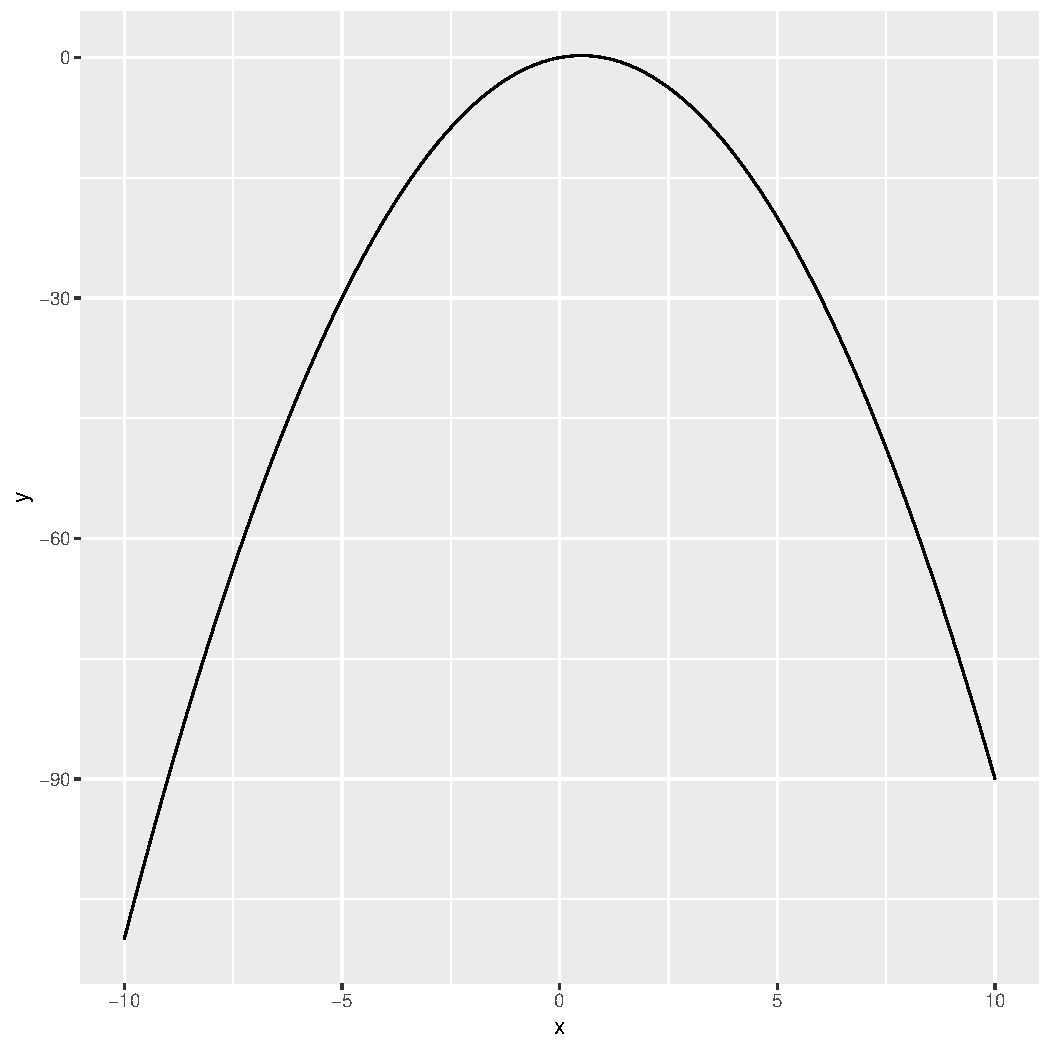
\includegraphics[width=\maxwidth]{figure/unnamed-chunk-3-1} 
\end{knitrout}
    \item This calculates the degrees of the vertex and places them in the vector \texttt{deg} and the number of edges in \texttt{edges}
\begin{knitrout}
\definecolor{shadecolor}{rgb}{0.969, 0.969, 0.969}\color{fgcolor}\begin{kframe}
\begin{alltt}
\hldef{deg} \hlkwb{=} \hlkwd{degree}\hldef{(ER_graph)}
\hldef{edges} \hlkwb{=} \hlkwd{gsize}\hldef{(ER_graph)}
\hldef{edges}
\end{alltt}
\begin{verbatim}
## [1] 32
\end{verbatim}
\end{kframe}
\end{knitrout}
    \item We plot the histogram now
\begin{knitrout}
\definecolor{shadecolor}{rgb}{0.969, 0.969, 0.969}\color{fgcolor}\begin{kframe}
\begin{alltt}
\hlkwd{hist}\hldef{(deg)}
\end{alltt}
\end{kframe}
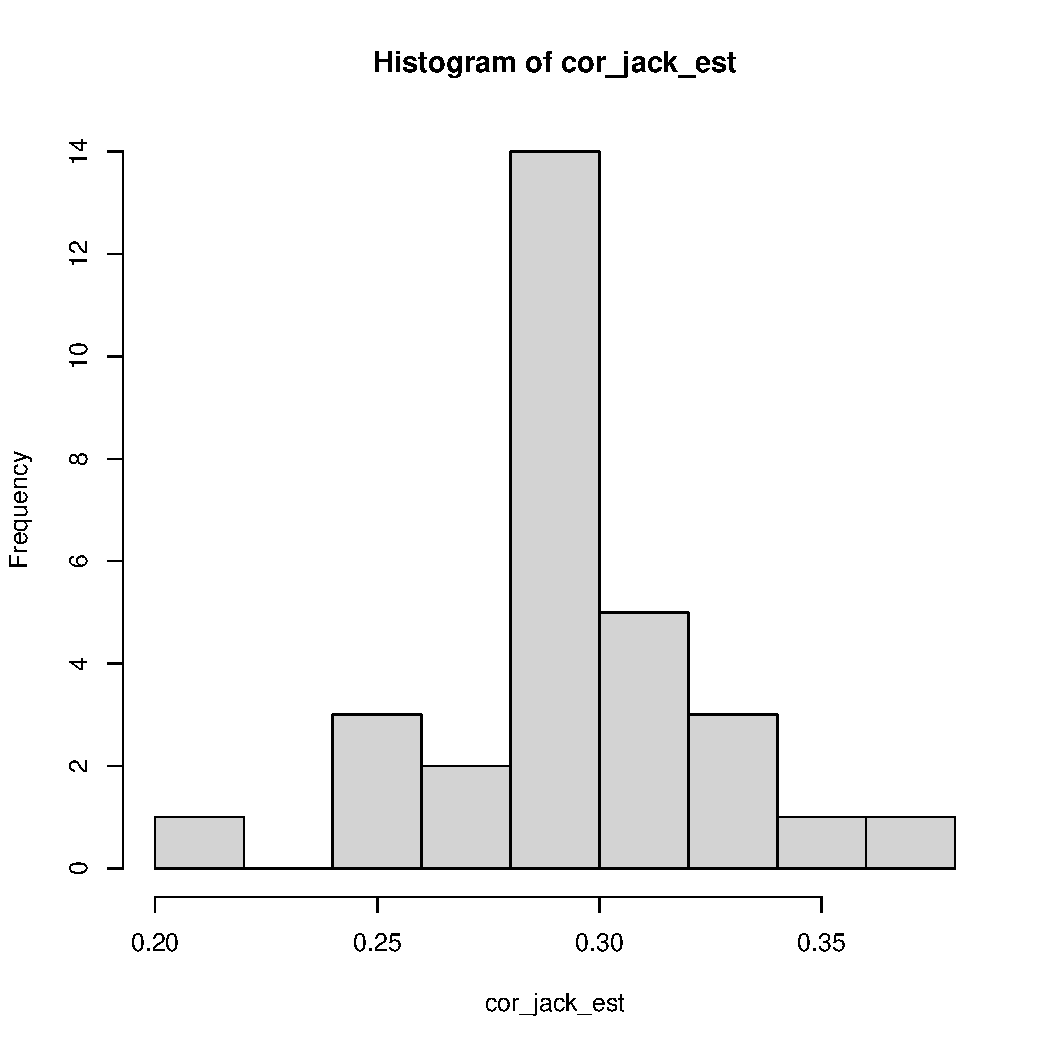
\includegraphics[width=\maxwidth]{figure/unnamed-chunk-5-1} 
\end{knitrout}
    \end{enumerate}
\item We set $p=4/6$ as in worksheet I and do the same
\begin{knitrout}
\definecolor{shadecolor}{rgb}{0.969, 0.969, 0.969}\color{fgcolor}\begin{kframe}
\begin{alltt}
\hldef{p} \hlkwb{=} \hlnum{4}\hlopt{/}\hlnum{6}
\hldef{prob_of_head} \hlkwb{<-} \hldef{p}
        \hldef{prob_of_head}
\end{alltt}
\begin{verbatim}
## [1] 0.6666667
\end{verbatim}
\begin{alltt}
        \hldef{prob_of_tail} \hlkwb{<-} \hlnum{1}\hlopt{-}\hldef{prob_of_head}
        \hldef{prob_of_tail}
\end{alltt}
\begin{verbatim}
## [1] 0.3333333
\end{verbatim}
\begin{alltt}
        \hldef{coin_toss_outcome} \hlkwb{<-} \hlkwd{sample}\hldef{(}\hlkwd{c}\hldef{(}\hlsng{"HEAD"}\hldef{,}\hlsng{"TAIL"}\hldef{),} \hlnum{1}\hldef{,} \hlkwc{prob} \hldef{=} \hlkwd{c}\hldef{(prob_of_head, prob_of_tail) )}
        \hldef{coin_toss_outcome}
\end{alltt}
\begin{verbatim}
## [1] "TAIL"
\end{verbatim}
\begin{alltt}
    \hldef{number_of_vertices}\hlkwb{<-} \hlnum{10}
    \hldef{adj_matrix} \hlkwb{<-} \hlkwd{matrix}\hldef{(}\hlnum{NA}\hldef{,} \hlkwc{nrow}\hldef{=}\hlnum{10}\hldef{,} \hlkwc{ncol}\hldef{=}\hlnum{10}\hldef{)}
\hlkwa{for}\hldef{(i} \hlkwa{in} \hlnum{1}\hlopt{:}\hldef{(number_of_vertices}\hlopt{-}\hlnum{1}\hldef{))\{}
  \hlkwa{for}\hldef{(j} \hlkwa{in} \hldef{(i}\hlopt{+}\hlnum{1}\hldef{)}\hlopt{:}\hldef{number_of_vertices) \{}
    \hlkwd{print}\hldef{(}\hlkwd{c}\hldef{(i,j))}
    \hldef{junk} \hlkwb{=} \hlkwd{sample}\hldef{(}\hlkwd{c}\hldef{(}\hlsng{"HEAD"}\hldef{,}\hlsng{"TAIL"}\hldef{),} \hlnum{1}\hldef{,} \hlkwc{prob} \hldef{=} \hlkwd{c}\hldef{(prob_of_head,prob_of_tail))}
    \hlkwa{if}\hldef{(junk}\hlopt{==}\hlsng{"HEAD"}\hldef{)}
    \hldef{adj_matrix[i,j]} \hlkwb{=} \hlnum{1}
    \hlkwa{else}
      \hldef{adj_matrix[i,j]}\hlkwb{=} \hlnum{0}
    \hldef{adj_matrix[j,i]} \hlkwb{=} \hldef{adj_matrix[i,j]}
  \hldef{\}}
\hldef{\};}
\end{alltt}
\begin{verbatim}
## [1] 1 2
## [1] 1 3
## [1] 1 4
## [1] 1 5
## [1] 1 6
## [1] 1 7
## [1] 1 8
## [1] 1 9
## [1]  1 10
## [1] 2 3
## [1] 2 4
## [1] 2 5
## [1] 2 6
## [1] 2 7
## [1] 2 8
## [1] 2 9
## [1]  2 10
## [1] 3 4
## [1] 3 5
## [1] 3 6
## [1] 3 7
## [1] 3 8
## [1] 3 9
## [1]  3 10
## [1] 4 5
## [1] 4 6
## [1] 4 7
## [1] 4 8
## [1] 4 9
## [1]  4 10
## [1] 5 6
## [1] 5 7
## [1] 5 8
## [1] 5 9
## [1]  5 10
## [1] 6 7
## [1] 6 8
## [1] 6 9
## [1]  6 10
## [1] 7 8
## [1] 7 9
## [1]  7 10
## [1] 8 9
## [1]  8 10
## [1]  9 10
\end{verbatim}
\begin{alltt}
\hlkwd{diag}\hldef{(adj_matrix)} \hlkwb{<-} \hlnum{0}
\hldef{ER_graph} \hlkwb{<-} \hlkwd{graph_from_adjacency_matrix}\hldef{(adj_matrix,}\hlkwc{mode}\hldef{=}\hlsng{"undirected"}\hldef{)}
\hldef{ER_graph}
\end{alltt}
\begin{verbatim}
## IGRAPH b1eeb4c U--- 10 35 -- 
## + edges from b1eeb4c:
##  [1] 1-- 3 1-- 4 1-- 5 1-- 6 1-- 7 1-- 8 1--10 2-- 5 2-- 6 2-- 7 2-- 9 2--10
## [13] 3-- 4 3-- 5 3-- 6 3-- 7 3-- 9 3--10 4-- 6 4-- 7 4-- 8 4-- 9 4--10 5-- 7
## [25] 5-- 8 5-- 9 5--10 6-- 7 6--10 7-- 8 7-- 9 7--10 8-- 9 8--10 9--10
\end{verbatim}
\begin{alltt}
\hlkwd{plot}\hldef{(ER_graph,} \hlkwc{edge.arrow.size}\hldef{=}\hlnum{0.5}\hldef{,} \hlkwc{vertex.color}\hldef{=}\hlsng{"#fde725"}\hldef{,} \hlkwc{vertex.size}\hldef{=}\hlnum{20}\hldef{,}
     \hlkwc{vertex.frame.color}\hldef{=}\hlsng{"#440154"}\hldef{,} \hlkwc{vertex.label.color}\hldef{=}\hlsng{"#440154"}\hldef{)}
\end{alltt}
\end{kframe}
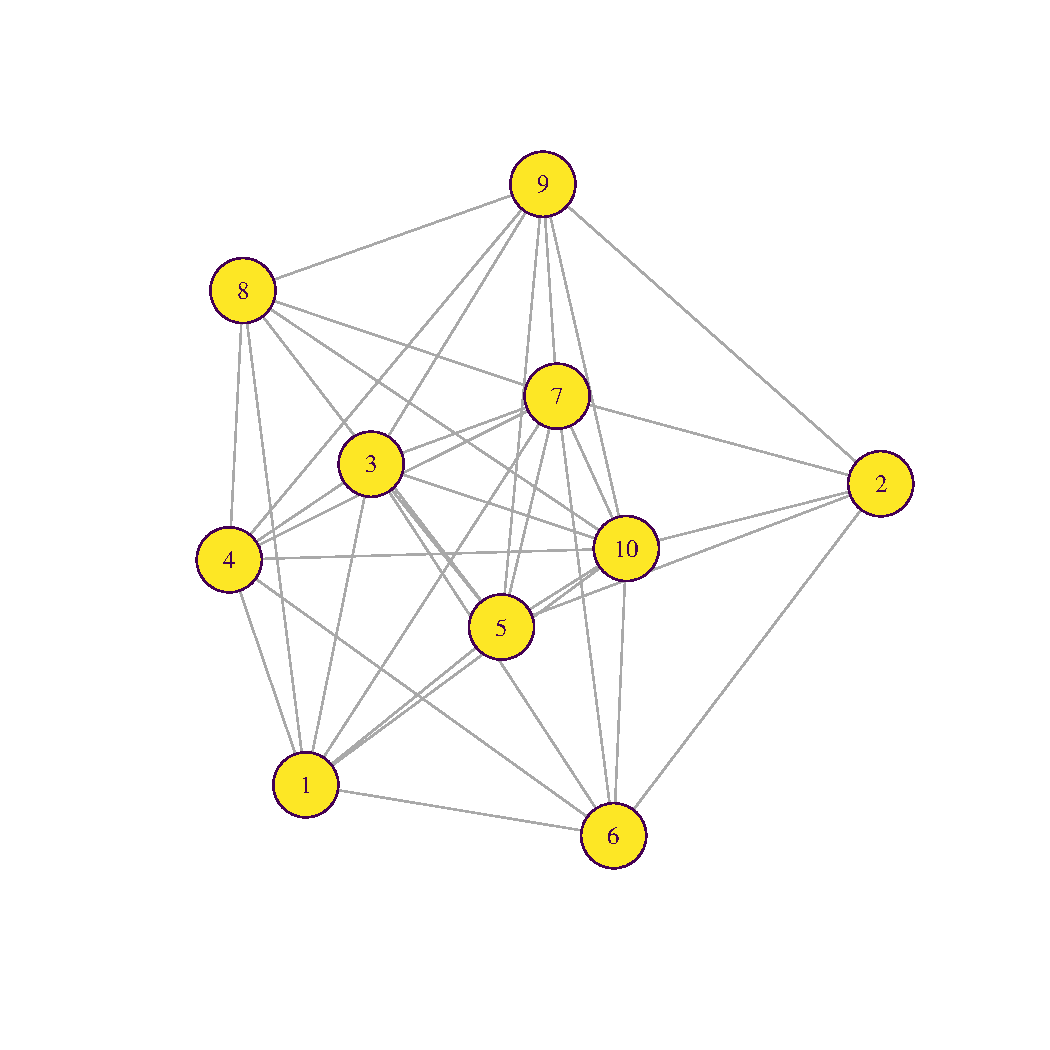
\includegraphics[width=\maxwidth]{figure/unnamed-chunk-6-1} 
\end{knitrout}
\end{enumerate}
\end{document}
